\documentclass[11pt]{article}
\usepackage{geometry} 
\geometry{a4paper,top=3cm,bottom=3cm,left=2.5cm,right=2.5cm}   
\usepackage{multicol}
\usepackage[english, italian]{babel}
\usepackage{fancyhdr}
\usepackage{musicography}
\geometry{centering}
\usepackage{graphicx}


\pagestyle{fancy}                                 %serve ad inserire la linea sopra e il titolino
\rhead{\textsf{Lezione 1 "\textit{Fondamenti di Max}"}}
\renewcommand{\headrulewidth}{5pt} %grandezza della linea in alto
\renewcommand{\footrulewidth}{1pt}   % grandezza della linea in basso


\begin{document}
\begin{minipage}{0.55\linewidth}
\vspace{0.3cm}
{\large{\textbf{\textsf{Gabriele Petrillo}}}}\\\end{minipage}

\vspace{0.3cm}
\begin{minipage}{0.95\linewidth}
\begin{center}
{\huge{\textbf{\textsf{Fondamenti di Max}}}} \\
\end{center}
\end{minipage}
\vspace*{0.2cm}


%=========ABSTRACT=======================
\begin{center}
\begin{minipage}[c]{14cm}
\begin{textit}

Questa prima lezione è dedicata allo studio dei fondamentali della programmazione in Max Msp.

\end{textit}
\end{minipage}
\end{center}
\vspace*{0.2cm}

%=========ARTICOLO========================

\begin{multicols*}{2}
\parskip=0pt

\textbf{\textsf {01 Patchcords}}\\

\noindent Max è un linguaggio di programmazione basato sul collegamento di oggetti grafici tramite cavi chiamati \textit {patch chords}. Gli \textit{object box} sono piccoli programmi che eseguono delle azioni di calcolo, tuttavia in Max sono presenti altre due tipologie di scatole chiamate \textit{message box} e \textit{comment box}: i primi sono messaggi alphanumerici che possono essere inviati o ricevuti da un object box, i secondi sono commenti che possiamo scrivere all’interno della patch.
A seconda del tipo di dati che gli object box spediscono i cavi di collegamento saranno di colore diverso: \textbf{grigi} dati numerici o stringhe, \textbf{gialli} per flussi di dati audio e \textbf{verdi} per il video.\\

\begin{center}
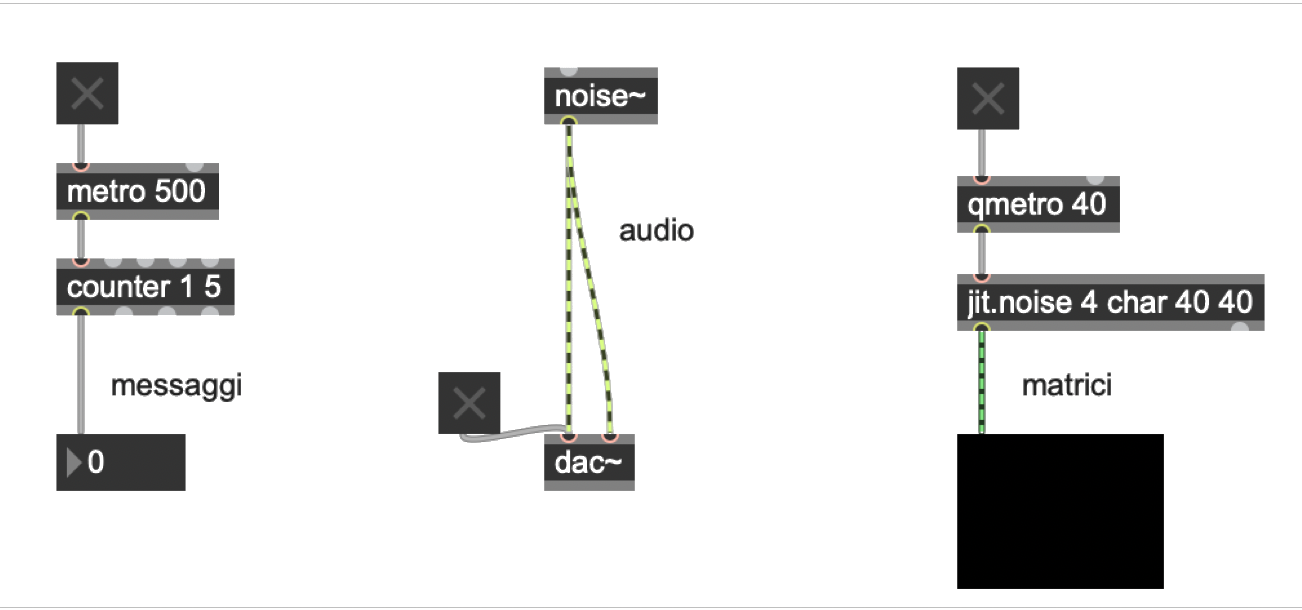
\includegraphics[scale=0.3]{images/01patchcords.png}

{\scriptsize \emph{fig.1 }}
\end{center}

\textbf{\textsf {02 Introduzione a Max}}\\

\noindent Il \textbf{bang} è un messaggio che ha il compito di dire agli oggetti di fare quello che devono fare, quindi inviare dei messaggi dai loro outlet. Può essere collegato a più oggetti o messaggi per ottenere un output multiplo.
L’oggetto \textbf{print} serve a visualizzare l’output di un messaggio o di un oggetto nella console di max, può essere chiamato con un nome specifico, ed ha una funzione di controllo.
Nella prima patch un \textbf{bang} è collegato a tre messaggi, collegati a loro volta all’oggetto \textbf{print A}. Se facciamo click sul bang possiamo vedere stampati nella console di Max i tre messaggi.
Gli oggetti \textbf{bangbang} e \textbf{trigger} servono ad indirizzare più messaggi di bang nel primo caso, messaggi vari nel secondo, in un certo ordine. L’argomento dell’oggetto \textbf{bangbang} è il numero di output desiderato, mentre quello di \textbf{trigger} è il tipo di messaggi che deve inviare in un determinato ordine. Una differenza importante è che l’oggetto \textbf{trigger} può ricevere un qualsiasi tipo di messaggio ed inviarlo da qualsiasi output implementato.\\

\begin{center}
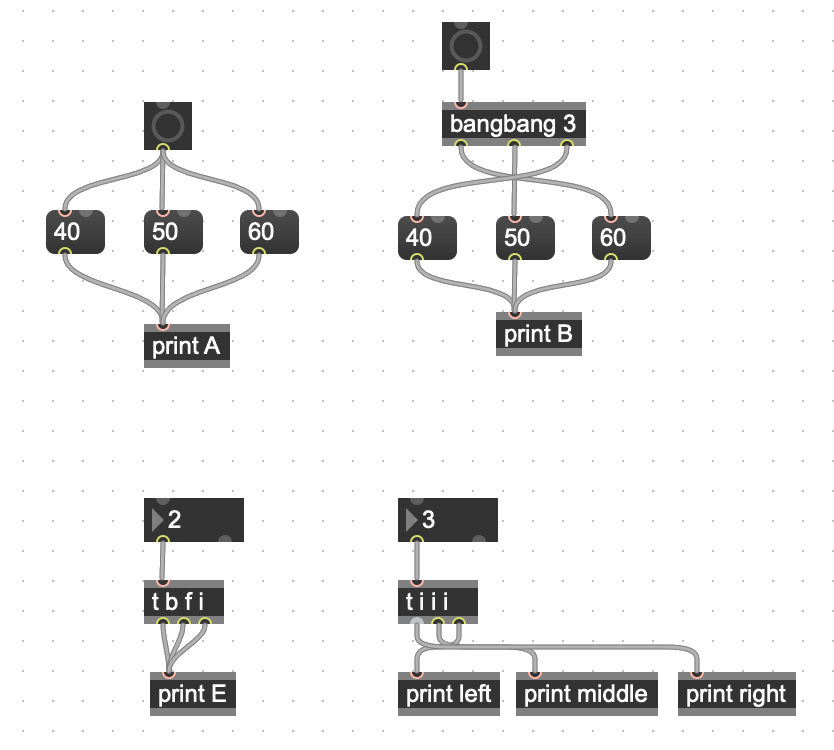
\includegraphics[scale=0.3]{images/02_bang.png}

{\scriptsize \emph{fig.2 }}
\end{center}

\textbf{\textsf {03 Number Box}}\\

\noindent Il \textbf{number box} è un oggetto che invia dei messaggi contenenti dei numeri. Esistono due tipi di Number box: \textbf{float} (numeri con la virgola) \textbf{int} (numeri interi). I numeri possono essere controllati tramite scroll, qualsiasi oggetto grafico come dial o fader, o scrivendoci dentro il numero. Ogni volta che cambiamo inseriamo un numero l’oggetto provoca un output del numero, tuttavia se vogliamo solo caricare il numero senza provocare nessun output bisogna inviare un messaggio con in numero preceduto dalla keyword \textit{set}.
Se colleghiamo un Number box ad un messaggio, possiamo avere un messaggio con un numero variabile inserendo nel messaggio la keyword “\$1”, per i numeri interi o “\$1.” per i numeri con la virgola.
La conversione di un numero di un tipo in un altro si chiama casting. Se convertiamo un numero int in un float, la conversione è senza perdite di informazione, viceversa perderemo tutti i numeri dopo la virgola.

\begin{center}
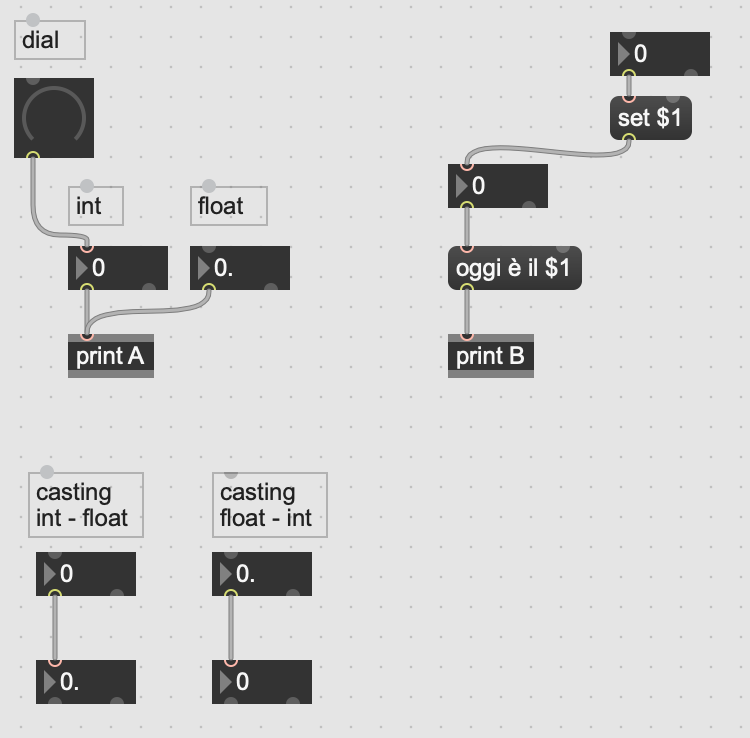
\includegraphics[scale=0.3]{images/03_number.png}

{\scriptsize \emph{fig.3 }}
\end{center}

\textbf{\textsf {04 Toggle e Metro}}\\

\noindent L’oggetto \textbf{toggle} di default invia uno 0 o un 1 e spesso è utilizzato come un interruttore per gli molti oggetti max. Tuttavia se inviamo un numero tramite messaggio a \textbf{toggle} questo lo lascerà passare facendo un casting in integer.
L’oggetto \textbf{metro} è un oggetto molto utile in max ed è utilizzato per sincronizzare il funzionamento di più oggetti e regolare la velocità di generazione degli eventi. Sostanzialmente è un metronomo che si avvia con un messaggio di \textit{1} e si spegne con \textit{0}. L’output dell’oggetto \textbf{metro} sono una serie di bang ad una velocità regolata per default in millisecondi e che può essere specificata o come argomento, o con un messaggio nell’inlet destro. Se colleghiamo più oggetti metro ad uno stesso messaggio di start possiamo azionare processi a velocità diverse parallelamente.

\begin{center}
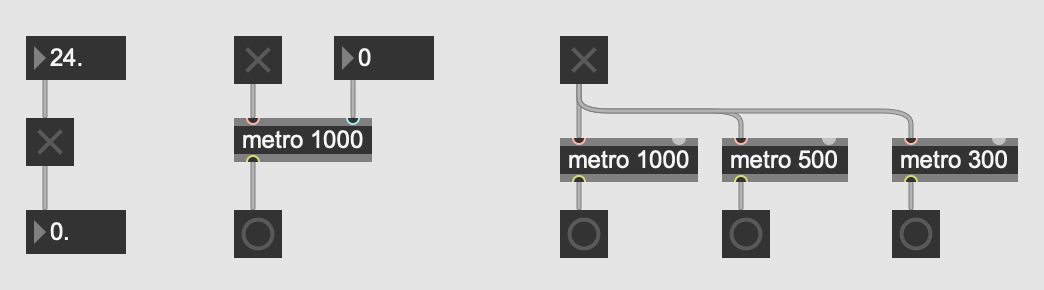
\includegraphics[scale=0.3]{images/04_toggle e metro.png}

{\scriptsize \emph{fig.4 }}
\end{center}

\textbf{\textsf {05 Ordine degli eventi e debug}}\\

\noindent Anche se può sembrare che max faccia più cose contemporaneamente, tutti i calcoli vengono fatti uno alla volta e in un certo ordine. È molto importante mettere gli oggetti nel giusto posto nella patch per far capire a max in che ordine fare i calcoli.
L’ordine di precedenza di max è destra - sinistra, basso - alto. Se ci sono dubbi è possibile verificare l’ordine dei messaggi con la funzione debug (nel menù in alto) applicando i watchpoint sui cavi. (per fare questo dobbiamo andare nel menù debug ed abilitare il debug, poi selezionare un cavo ed inserire il watchpoint desiderato)
Per ovviare al problema grafico del posizionamento degli oggetti possiamo usare l’oggetto “trigger” che dato un certo input (qualsiasi messaggio alphanumerico” può gestire l’ordine di output di determinati eventi.

\begin{center}
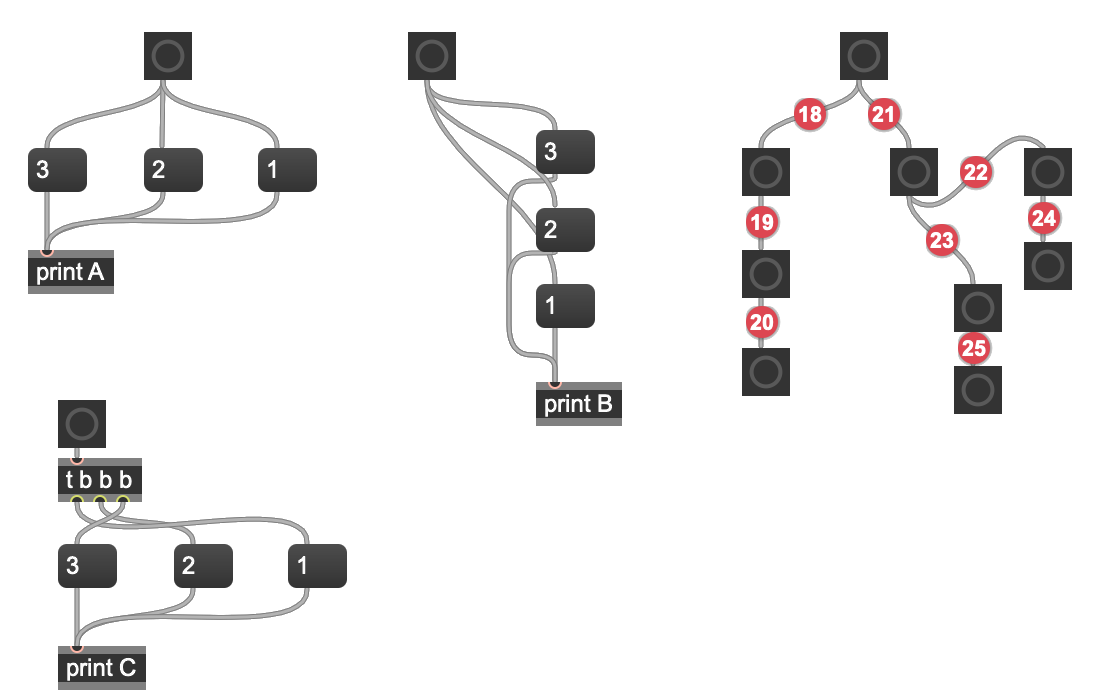
\includegraphics[scale=0.3]{images/05_debug.png}

{\scriptsize \emph{fig.5 }}
\end{center}

\textbf{\textsf {05 Liste}}\\

\noindent Per lista si intende un messaggio contenente una serie di dati alphanumerici. Le liste sono utili per inviare variabili con Keyword agli oggetti o far camminare più informazioni contemporaneamente per poi essere divise.
Gli oggetti che ci permettono di creare o spacchettare liste sono “pack” “pak” e “unpack”. I primi due servono a creare liste, come argomento vanno inseriti i tipi di dato che devono ricevere dagli inlet rispettivi, la differenza tra i due oggetti è che il primo ha solo il primo inlet caldo, mentre il secondo gli ha tutti. L’oggetto “unpack” serve a spacchettare una lista in più messaggi singoli e come argomento richiede i tipi di messaggi che deve spacchettare dall’outlet rispettivo.
Per creare dei messaggi contenenti delle liste possiamo utilizzare gli oggetti “append” e “prepend” che come argomento vogliono il messaggio da inserire dopo o prima del messaggio arrivato dall’inlet. Se nella messaggio sono contenute virgole, Max interpreterà quel messaggio come due stringhe.

\begin{center}
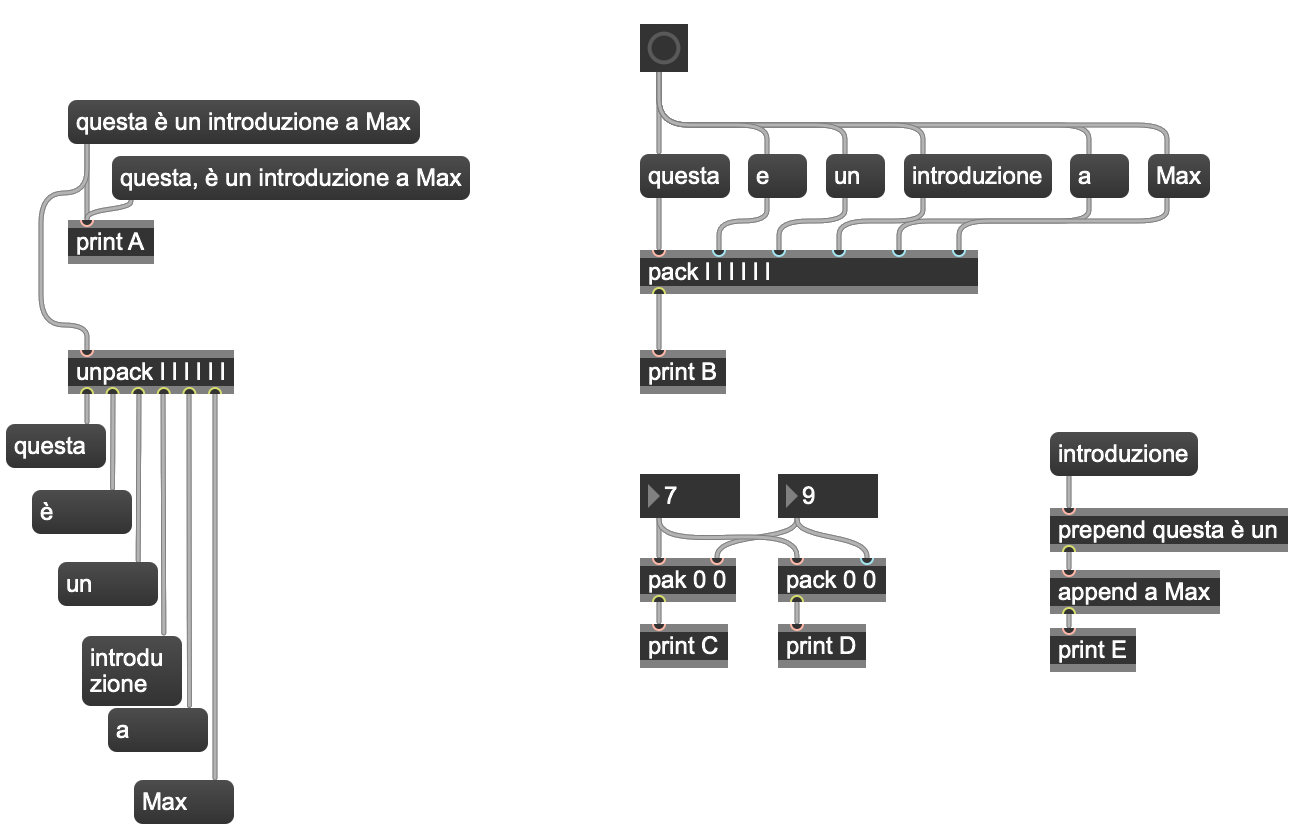
\includegraphics[scale=0.3]{images/06_liste.png}

{\scriptsize \emph{fig.6 }}
\end{center}


\section*{\centering\small{BIBLIOGRAFIA}}
•\textsc{\textsf {Cipriani, Alessandro and Giri Maurizio}}, \emph{Musica Elettronica e Sound Design}, Contemponet 2012\\

\end{multicols*}

\end{document}